
%(BEGIN_QUESTION)
% Copyright 2014, Tony R. Kuphaldt, released under the Creative Commons Attribution License (v 1.0)
% This means you may do almost anything with this work of mine, so long as you give me proper credit

Beregn alle spenninger og alle strømmer i denne transformatorkretsen, gitt at kilden leverer 4.5 ampere til transformatorens primærvikling:

$$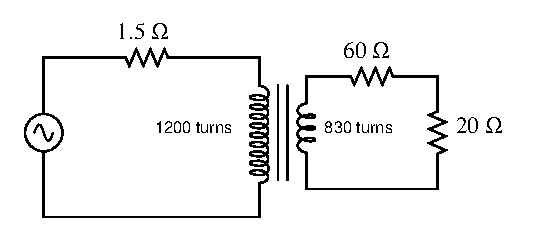
\includegraphics[width=15.5cm]{i01268x01.eps}$$

\begin{itemize}
\item{} $V_{source}$ = 
\item{} $V_{primary}$ = 
\item{} $V_{secondary}$ = 
\item{} $I_{primary}$ = 
\item{} $I_{secondary}$ = 
\end{itemize}

\vfil 

\underbar{file i01268}
\eject
%(END_QUESTION)





%(BEGIN_ANSWER)

Dette er et vurdert spørsmål -- ingen svar eller hint er gitt!

%(END_ANSWER)





%(BEGIN_NOTES)

\begin{itemize}
\item{} $V_{source}$ = 759.3 volt
\item{} $V_{primary}$ = 752.5 volt
\item{} $V_{secondary}$ = 520.5 volt
\item{} $I_{primary}$ = 4.5 ampere
\item{} $I_{secondary}$ = 6.506 ampere
\end{itemize}

%INDEX% Electronics review: transformer ratios

%(END_NOTES)

